%
% File acl2020.tex
%
%% Based on the style files for ACL 2020, which were
%% Based on the style files for ACL 2018, NAACL 2018/19, which were
%% Based on the style files for ACL-2015, with some improvements
%%  taken from the NAACL-2016 style
%% Based on the style files for ACL-2014, which were, in turn,
%% based on ACL-2013, ACL-2012, ACL-2011, ACL-2010, ACL-IJCNLP-2009,
%% EACL-2009, IJCNLP-2008...
%% Based on the style files for EACL 2006 by 
%%e.agirre@ehu.es or Sergi.Balari@uab.es
%% and that of ACL 08 by Joakim Nivre and Noah Smith

\documentclass[11pt,a4paper]{article}
\usepackage[hyperref]{acl2020}

\usepackage{amsmath}
\usepackage{amsfonts}
\usepackage{amssymb}
\usepackage{booktabs}
\usepackage{color, colortbl}
\usepackage{enumitem}
\usepackage{graphicx}
\usepackage{hyperref}
\usepackage[latin1]{inputenc}
\usepackage{latexsym}
\usepackage{multirow}
\usepackage{times}
\usepackage{url}
\usepackage{xcolor}
\usepackage{xspace}

\renewcommand{\UrlFont}{\ttfamily\small}

%\usepackage{microtype}

%\aclfinalcopy % Uncomment this line for the final submission
%\def\aclpaperid{***} %  Enter the acl Paper ID here

%\setlength\titlebox{5cm}
% You can expand the titlebox if you need extra space
% to show all the authors. Please do not make the titlebox
% smaller than 5cm (the original size); we will check this
% in the camera-ready version and ask you to change it back.

\newcommand{\sz}[1]{\textcolor{blue}{\emph{//sz: #1//}}}
\newcommand{\gbt}[1]{\textcolor{orange}{\emph{//gbt: #1//}}}
\newcommand{\cs}[1]{\textcolor{green!60!black}{\emph{//cs: #1//}}}
\newcommand{\mw}[1]{\textcolor{orange!60!black}{\emph{//mw: #1//}}}

% To streamline frequently used terms:
\newcommand{\langvis}{language\ \&\ vision\xspace}
\newcommand{\lv}{L\&V\xspace}
\newcommand{\mn}{ManyNames\xspace}
\newcommand{\vg}{VisualGenome\xspace}

\newcommand{\cat}[1]{\textsc{#1}}
\newcommand{\name}[1]{\textsl{#1}}

\title{How to Name a Real-World Object, and how not to}

\author{First Author \\
  Affiliation / Address line 1 \\
  Affiliation / Address line 2 \\
  Affiliation / Address line 3 \\
  \texttt{email@domain} \\\And
  Second Author \\
  Affiliation / Address line 1 \\
  Affiliation / Address line 2 \\
  Affiliation / Address line 3 \\
  \texttt{email@domain} \\}

\date{}

\begin{document}
\maketitle
\begin{abstract}

\end{abstract}

\section{Introduction}
\label{sec:intro}
Objects, being members of many categories, can be called by many names (e.g.,\ a duck can be called \name{duck, bird, animal} etc.). 
The task of \emph{object naming} -- generating not just a formally correct but also an appropriate, \emph{natural} name for an object -- is distinct from the closely related tasks of object detection and image classification (see below).
It has been studied in psycholinguistics~\cite{refs} \mw{Refs!}, but has received comparatively little attention in \langvis (\lv) and computational linguistics (CL) research.
We address the following question:\\
\fbox{\parbox{\columnwidth}{\textbf{Q:} Can standard object detection/image classification models (be fine-tuned to) exhibit human-like object naming behavior?}}\\\\
In particular, we test several models for their ability to generate \emph{entry-level names}, i.e., the names people prefer when calling a specific object (e.g.,~\name{duck} in Figure~\ref{fig:duck}, right image).
We wish to find out, for instance, whether different types of models or training regimes will tend towards different kinds of human-like errors in this regard.
A secondary contribution of this paper is instrumental: for a proper evaluation we must first augment an existing human object naming dataset (\mn, Anonymous, under review) with extensive quality control, the resulting data of which we also describe and make available with this paper.

In \lv, the choice of a particular name for an object is a ubiquitous problem -- it underlies virtually all tasks that model how speakers use language to refer to objects in the world, such as image description, visual question answering and referring expression generation.
\lv methods are generally based on object detection or image classification models from computer vision (CV) research (or the visual features extracted from them) that were pre-trained towards predicting the single label of each object that is deemed correct by the dataset.
The labels used often seem unintuitive from a human perspective, e.g., some are very basic, natural names (e.g., \name{bus}) while others seem overly specific (e.g.,\ \name{goblet, gyromitra}; cf.\ the label inventory of the ILSVRC challenges; \citealt{ILSVRC15}).
Pre-training on such labels has its justification in that computer vision models can learn rich, discriminative visual feature representations which capture fine-grained differences in object appearances (e.g.,\ sharp-pointed vs. slightly pointed). 
But it raises the issue of whether these models could be used for more human-like object naming.
% Accordingly, these CV models are assessed by their ability to predict a single, in cases very specific, ground-truth label.

% By contrast, the goal of \lv object naming models is to predict the `natural' name of an object, i.e.,~the name a human could choose for the object instance.
Psycholinguistic studies have found that humans have a preference towards a particular name, defined as the \textit{entry-level name}, when naturally naming an object \cite{rosch1976basic,Rosch1978,jolicoeur1984pictures}. 
However, this research has traditionally focused on \categories and/or their prototypical/schematic depictions (e.g., \newcite{rossion2004revisiting}), as opposed to the situated instances in naturalistic images with which \lv is mostly concerned.
Humans may prefer different names for different instances of the same \category, and have them even disagree in their choice for the same instance (see also \citealt{graf2016animal}).
For example, in Figure~\ref{fig:duck}, for the two instances of a duck (from \vg, with names from \mn), most people (27 out of 36) called the instance on the left \name{bird}, while \name{duck} was strongly preferred for the right instance. 
\begin{figure}[t]
	\centering
	\small
	\begin{tabular}{p{3cm}p{3cm}}
		\centering
		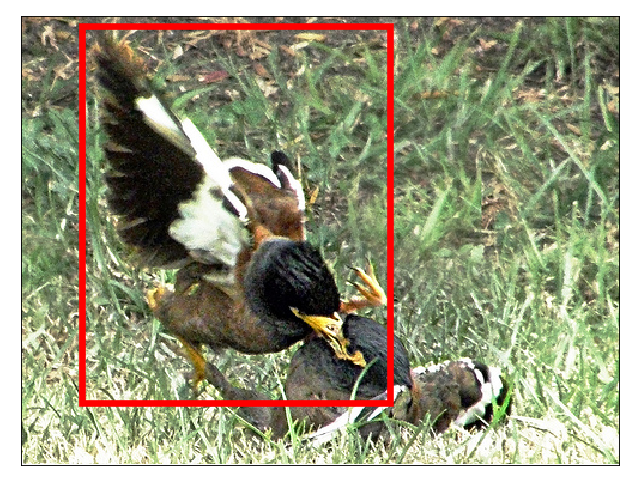
\includegraphics[scale=0.15]{images/2327551_2960743_seed_ambiguous.png} &
		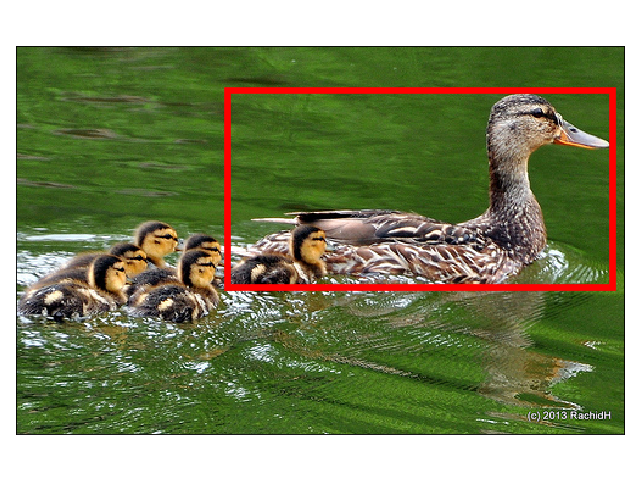
\includegraphics[scale=0.15]{images/2358126_805887_singleton_obj.png}\\
		bird\ (27),  duck\ (8) & duck (33), bird (3)\\
	\end{tabular}
	\caption{Different naming preferences for different instances of the same \category \name{duck} in \mn.\label{fig:duck}}
\end{figure}
Hence, both the single-ground-truth view of CV models and the category-level approach predominant in Psycholinguistics are insufficient for assessing the effectiveness of \lv models for human-like, entry-level object naming.
The \mn dataset was designed to help mend this gap: it consists of names entered by 36 annotators in parallel, for 25K objects in naturalistic images from \vg~\cite{krishna2016visualgenome}.
However, the name annotations of \mn have not been verified to filter out incorrect names or names for the wrong object, a problem that is in some sense the opposite of that posed by the single-ground-truth approach.

Our main contributions in this paper are (i) to run the \mn data through a rigorous annotation round to quantify both the adequacy of its names and the types of errors they contain, in order to (ii) test and compare object detection and image classification models for their ability at the task of \emph{instance-based, entry-level object naming}. More precisely, \mn enables us to define the entry-level as follows:\\
\fbox{\parbox{\columnwidth}{\textbf{Entry-level name:} the most common name given to an object instance according to \mn}}\\\\
We evaluate the effectiveness of different models on predicting these entry-level names, and our additional verification annotations enable us to understnad the kinds of mistakes each model makes (e.g.,~a `wrong' prediction may be a less preferred name as opposed to a true error).
We show that generic object classification models on their own (ResNet, Faster-RCNN and Bottom-up) already learn to provide entry-level names for objects, but also that it is possible to apply transfer learning on \mn, successfully using pre-trained features from object detection and image classification models to train entry-level naming models. 
\mw{Remark about the kinds of human errors, just as in the abstract, or some other more interesting teaser?}

%% END OF FILE %%

%Our contributions towards the task of instance-based entry-level naming in \lv and CL research are two-fold:  
%First, we provide data on object naming with real images on a large scale. 
%We take on an empirical notion of entry-level names, and define it on the instance-level, i.e., the name that humans prefer to use when calling a particular object in a real-world image.   
%We extend \mn (under submission), a dataset that provides 36 names for each of 25K objects from \vg~\cite{krishna2016visualgenome}, with information on adequacy and reference of all collected names, which affords rich analysis possibilities. 
%
%Second, we introduce the verified \mn dataset as evaluation data, and provide an extensive analysis of the ability of object detection and classification models to account for entry-level object naming in our dataset. 


\iffalse
%However, when they speak, humans in general name specific \textit{instances} of objects---actually, instances in particular situations and points of view, which may humans have prefer different names for instances of the same \category, and have them even disagree in their choice for the same instance (see also \citealt{graf2016animal}). 


%Accordingly, datasets used for object naming in Psycholinguistics use idealized drawings that correspond more to categories than to instances~\cite{+++++}.
%
%

Despite its relevance in \lv and CL, the challenge of instance-based natural naming has been overseen. 
\lv research that particularly focuses on the prediction of entry-level names is scarce, and existing work has adopted the \category-based concept of entry-level names \cite{Ordonez:2016}. 
Furthermore, existing datasets lack necessary information to make progress in \lv and CL research on this phenomenon. 
\cs{TODO@CS: EVALUATION ISSUE GOES HERE.}
\begin{itemize}
	\item resources developed in CV and \lv can be useful to study object naming. 
	\item However, they provide only one (or a few) name per object \ra no guarantee that it is the entry-level name. (We provide more, to have a robust estimate of entry-level names (as well as data on other possible names). \gbt{actually, maybe move this to the previous part? \ra differences with Psycholing, with CV resources})
	\item object naming has often been conflated with object classification in CV. \gbt{Discuss differences; mention the swan - whatever name it has in wordnet example of ordonez et al?}
	\item a big problem with this approach is that it follows a single-label evaluation. With our data, we show that often model responses are adequate even if they do not correspond to the entry-level name.
	\item we also show that object classification models ``spontaneously'' learn to provide entry-level names for objects
	\item and that it is possible to use \mn to successfully fine-tune existing object detection and classification models to predict entry-level names for objects.
\end{itemize}


This paper seeks to spur \lv and CL research on the problem of \textit{instance-based entry-level object naming}. 

Our contributions are two-fold:  
First, we provide data on object naming with real images on a large scale. 
We take on an empirical notion of entry-level names, and define it on the instance-level, i.e., the name that humans prefer to use when calling a particular object in a real-world image.   
We extend \mn (under submission), a dataset that provides 36 names for each of 25K objects from \vg~\cite{+++}, with information on adequacy and reference of all collected names, which affords rich analysis possibilities. 

\cs{I'll continue from here.}
Second, we introduce the verified \mn dataset as evaluation data that allows XXX. We provide an extensive analysis of the ability of object detection and classification models on the task of predicting the entry-level names in our dataset.


When people talk, they choose particular names for objects, such as \textit{bird} or \textit{duck} for the images in Figure~\ref{fig:duck}.
The task of \textbf{object naming} has been studied in Psycholinguistics~\cite{refs}, \gbt{Which term do you prefer, Psycholing, or CogSci? I don't care. Use same term throughout.} but has not received much attention in Computational Linguistics; we seek to remedy this situation by providing data and modeling results on this phenomenon, and in particular on \textbf{entry-level names}, defined in psycholinguistic research as the preferred name for an object~\cite{rosch1976basic,Rosch1978,jolicoeur1984pictures}: For the left object in the figure, according to our data, the entry-level name is \textit{bird}, and for the right object it is instead \textit{duck}.
%We seek to shed light into how people naturally name objects in real images, and in 


Our contributions are two-fold.
First, we provide data on object naming with real images on a large scale.
We extend \mn (under submission), a dataset that provides 36 names for each of 25K objects from \vg~\cite{+++}, with information on adequacy and reference of all collected names, which affords rich analysis possibilities. 
Our data contain object instances, corresponding more closely to the kind of visual objects that humans typically encounter, and so can potentially shed light on the instance-level factors that affect naming. 

Second, we provide an extensive analysis of the performance of object classification models on the task of predicting the entry-level names in our dataset.

As for the former, note that Psycholinguistic research on entry-level names has focused on categories, as opposed to instances:
When a subcategory is atypical, such as penguins not being very typical birds, this affects their entry-level name (it is common to call a sparrow, but not a penguin, \textit{bird}).
Accordingly, datasets used for object naming in Psycholinguistics use idealized drawings that correspond more to categories than to instances~\cite{+++++}.
However, when they speak, humans in general name specific \textit{instances} of objects ---actually, object instances in particular situations and points of view.
Our data contain object instances, corresponding more closely to the kind of visual objects that humans typically encounter, and so can potentially shed light on the instance-level factors that affect naming.
%Indeed, Psycholinguistic research has typically ignored
% The example shows two instances of the category \textsc{duck}, and when people were asked to name the highlighted object, most ($27$) people called the instance on the left \name{bird}, while \name{duck} was strongly preferred for the right instance. 
%It seems plausible that there are instance-specific factors affecting naming behavior in general.
%, and entry-level names in particular, and our data suggest that this is the case
% gbt: maybe put back a "crucially" somewhere: "Crucially, though, as we will empirically show, human object naming is \textit{instance}-dependent: It depends on the characteristics "
In particular, we validate the notion of entry-level name at the instance level:
For almost 90\% of the 25K objects analyzed, humans showed a preference for a given name (frequency of that name $>50\%$ of the valid responses).

As for the second contribution, \gbt{to be expanded; proposed structure follows; probably here only a summary and a fuller explanation later?}
% allows for an in-depth analysis of naming data as well as of naming models on the task of object naming.
\begin{itemize}
\item resources developed in CV and \lv can be useful to study object naming. 
\item However, they provide only one (or a few) name per object \ra no guarantee that it is the entry-level name. (We provide more, to have a robust estimate of entry-level names (as well as data on other possible names). \gbt{actually, maybe move this to the previous part? \ra differences with Psycholing, with CV resources})
\item object naming has often been conflated with object classification in CV. \gbt{Discuss differences; mention the swan - whatever name it has in wordnet example of ordonez et al?}
\item a big problem with this approach is that it follows a single-label evaluation. With our data, we show that often model responses are adequate even if they do not correspond to the entry-level name.
\item we also show that object classification models ``spontaneously'' learn to provide entry-level names for objects
\item and that it is possible to use \mn to successfully fine-tune existing object detection and classification models to predict entry-level names for objects.
\end{itemize}

\gbt{Below is the old text. I factored out the entry-level aspects in the previous paragraph. It should be removed from this second part.}

Objects, being members of many categories, can be called by many names (e.g.,\ a duck can be called \name{duck, bird, animal} etc.). 
In \langvis research (\lv), the choice of a particular name for an object is a ubiquitous problem---it underlies virtually all tasks that model how speakers use language to refer to objects in the world, such as image description, visual question answering, referring expression generation, etc. 
%
\lv methods are generally based on object detection or image classification models (or the visual features extracted from them) that were pre-trained towards predicting the single correct label of objects. 
The set of labels are often determined rather arbitrarily---it may contain very specific (e.g.,\ \name{goblet, gyromitra}) as well as "basic-level" labels (e.g., \name{bus}; cf.\ the label inventory of the ILSVRC challenges; \citealt{ILSVRC15}). 

This pre-training strategy has its justification in that computer vision models can learn rich, discriminative visual feature representations which capture fine-grained differences in object appearances (e.g.,\ sharp--pointed vs. slightly pointed). 
It is, however, different from predicting the natural name of an object, 
because, as has been found in numerous studies in psychology, humans have a preference towards a particular name (\textit{entry-level name}, e.g.,\ \name{duck}) when naturally calling an object  \cite{rosch1976basic,Rosch1978,jolicoeur1984pictures}. 
Entry-level names have hereby usually been considered to be an attribute of concrete \textit{concepts} (e.g.,\ penguin, duck), where the choice of a concept's entry-level name depends on factors such as its typicality with respect to its basic-level category (bird). \cs{Need to check Jolicoeur and their experiments} 
Crucially, though, as we will empirically show, human object naming is \textit{instance}-dependent---contextual visual features may humans have prefer different names for object instances of the same concrete concept, and have them even disagree in their choice for the same instance (see also \citealt{graf2016animal}). 
For example, Figure~\ref{fig:duck} shows two instances of the concept duck, and when people were asked to name the highlighted object, most ($27$) people called the instance on the left \name{bird}, while \name{duck} was strongly preferred for the right instance. 

Despite its relevance in \lv, the challenge of instance-based natural naming has been overseen, and most \lv datasets not necessarily provide enough information to make progress on the problem of modeling natural object naming (they only provide very few names). 
Research that particularly focuses on the prediction of entry-level names is scarce, and existing work has adopted the view that (i) entry-level names arise on the conceptual level, and (ii) developed specialized methods \cite{Ordonez:2016}. 
%To our knowledge, work that gives systematic insights into the ability of standard object recognition models to account for natural object naming, and in how far simple \cs{straightfoward?} re-training or transfer learning can increase this ability, is lacking. 
%

In this paper, we seek an understanding of the notion of entry-level names of instances of real-world objects in images, and to give systematic insights into the problem of retraining or fine-tuning object detection models (and features in transfer learning) such that they capture a natural vocabulary and account for linguistic preferences in naming. %, i.e.,\ the name that humans naturally prefer to call an object.  
Specifically, and in contrast to previous works, we 
(i) take on an empirical notion of entry-level names, and define it on the instance-level, i.e., the name that humans prefer to use when calling a particular object in a real-world image.   
(ii) We examine in how far standard models in computer vision, namely object detection and image classification models, do learn entry-level naming by being trained on images labeled with rather \textit{\arbitrary} (as opposed to entry-level) object names. \cs{add sth based on results - how to fine-tune or whether it's possible to fine-tune; how readily available they are to be used for transfer learning, the standard method in \lv}

We use \mn, a new dataset of real-world images, built on top of \vg, which provides an excellent resource for our study, since it was annotated with a large number\ $(36)$ of object names by means of a crowdsourcing study.

Our contributions are: 
(i) We present our extension of the \mn dataset that augments all collected object names with verification information, which allows an in-depth analysis of naming models on the task of object naming. 
(ii) Theoretical:
(a) We show that entry-level names should be derived on the instance-level as opposed to the XXX level \cs{(TO SHOW: entry-level names are different for the same "class" @Sina or @Matthijs?) (contrast to psychological studies)}
(b) We need many name annotations to derive the entry-level name (contrast to few annotations in L+V and computer vision; \cs{TO SHOW: entry-level name of an instance varies depending on the number of annotations/instance)}
(iii) Technical:
(a) Object detectors trained on "\arbitrary" natural object names do learn entry-level names to some extend (as expected: they learn the shared features leading to entry-level \cs{-- can we show that mistakes are rather class-based? i.e., tendency towards a certain name for each class?)}
(b) To predict entry-level names without annotating a huge amount of training examples, it is possible to fine-tune (iii) on \mn. We show that \cs{(say something about mistakes not made anymore). }

\fi
%%% Local Variables:
%%% mode: latex
%%% TeX-master: "acl2020_main"
%%% End:


\section{Related Work}
\label{sec:related}
%
%\paragraph{(Entry-Level) Object Naming}
%cognitive science/psychology:\\
%- levels of specificity\\
%- basic-level vs. entry-level\\ 
%- object naming studies
%
%Language + Vision:\\
%Ordonez et al., Zarriess \& Schlangen, ... \\
%- Our work: empirical notion of entry-level
%\cs{Necessary to say something about class vs. category? Otherwise I would just always use class to make things easier.}
%% SHORTENING %%Our work on natural object naming connects research in psycholinguistics, \langvis and computer vision. 
In psycholinguistics, studies of picture naming have found that humans identify objects at a preferred level of abstraction, the so-called basic-level \cite{rosch1976basic,jolicoeur1984pictures}. 
The typicality of the object with respect to this basic-level is important for determining the preferred name, i.e.\ the entry-level name: typical objects (e.g.,\ a robin) are simply named by their basic-level \category (\name{bird}), while atypical objects (e.g.,\ \name{penguin}) are preferably named by the more specific \category.
%% This strictly taxonomic view suggests that entry-level names generally hold for all instances of a \category (e.g.,\ penguin).   \mw{Not true!!}
\newcite{Ordonez:2016} adopt this and train a model to map an object's \category detected by an object recognition system to its natural name, guided by external resources like corpus statistics.
By contrast, we use \mn (details below) to directly test and fine-tune object recognition (and image classification) systems, without presupposing a taxonomical relationship between the possible names for an object.

Our approach is closer in this regard to \newcite{zarriess-schlangen:2017}, who train an object naming model from names produced in referring expressions to real-world objects.
However, they do not have access to name annotations from (many) different annotators, and they rely on simple evaluation measures (like accuracy) whereas the additional annotations we collect enable more fine-grained evaluation.
The \mn dataset on which we rely is akin in spirit to older picture naming datasets (e.g.,~\newcite{rossion2004revisiting}) but focuses on naturalistic images of real-world objects instead of prototypical line drawings.

 %\sz{maybe we should not mention the Graf paper here ... we do not look at objects in context}
 
%members of different \textit{basic-level} categories (e.g., a duck, a robin, a penguin, etc. are all members of \cat{birds}) 
% \newcite{rohde2012communicating} and \newcite{graf2016animal} investigate naming in context and find that the specificity of a name is dependent on the taxonomic relatedness of other objects in context.

%% SHORTENING %% \cs{Need to check Jolicoeur and their experiments; say sth about shared visual features}
% prototypical visual features common to all its instances (e.g.,\ apples are round, pears are ... (CHECK)). 

In Computer Vision a major focus is visual object recognition, with object classification being a core task. 
Neural image classification systems are trained to label the most salient object in an image and often use the ImageNet \cite{imagenet_cvpr09} benchmark that labels images/objects with 1,000 fine-grained classes \cite{googlenet,he2016deep}. 
These neural classifiers have proven extremely useful %% SHORTENING %%in a large range of transfer learning scenarios. They are commonly used 
as pre-trained feature extractors in object detection systems that localize objects and predict their labels \cite{fasterrcnn2015}.
For instance, a commonly used object detector in \lv is \citep{anderson2018updown}'s so-called bottom-up model, which is based on a pre-trained ResNet classifier and fine-tuned Faster-RCNN \cite{fasterrcnn2015} for object detection and classification on \vg. 
We will use pre-trained ResNet, Faster-RCNN and Bottom-up as models in this paper, extending and testing them for entry-level object naming. 

\paragraph{The ManyNames Dataset}
The \mn dataset (MN, Anonymous, under review) which builds upon object annotations in VisualGenome (VG), provides up to 36 name annotations for 25K objects in images, see e.g.\ Figure \ref{fig:duck}.
The large number of name annotations per object in \mn gives us a way to reliably derive entry-level names, defined as the most frequent name for an object instance.
Its vocabulary of all names has 7,970 types; restricted to entry-level names it has 442 types (still covering over 50\% of the objects in \vg).
	%% SHORTENING %%The vocabulary of all entry-level names in \mn contains 442 types (the vocabulary of all names is 7970), covering more than 50\% of the objects in \vg, i.e. almost 2M objects in \vg are mentioned in region descriptions with one of these 442 entry-level names.
That these objects are diverse and visually situated in real-world scenes aligns with our view that entry-level names should be characterized at an instance-level, not at the class-level.
However, our manual inspection of the \mn data revealed a range of annotation problems, e.g., annotators occasionally named an object different from the one highlighted by the bounding box, or the right object but with an incorrect name.
Although these errors are interesting human data, many of them would not occur in actual language use but are artifacts of the crowdsourcing methodology that uses simple graphical boxes to point workers to the annotation target.
%used for \mn, where there is a financial incentive to complete the task as quickly as possible.
As such they pose challenges for our research goal, which is to see whether the object-naming ability of computational models resembles that of actual language users.
To overcome these we collected a new layer of verification annotations on top of \mn, as follows.

%Current recognition benchmarks use labels (and images) from the ImageNet \cite{imagenet_cvpr09} taxonomy, but typically implement a single ground-truth label approach.
%- Object detection, using pre-trained feature representations (see next point) (localize object and predict its \textit{label}; trained with, e.g.\ more coarse-grained ImageNet labels or VG names)\\
%- Pre-trained feature representations, trained on image classification with 1000 ImageNet fine-grained labels (predict \textit{label} for most salient object in image). It predicts the class of the most salient object in an image. \\
%- Our work: can object detectors account for natural human object naming with respect to predicting the entry-level name? 

[Sectioning to be revised]

\paragraph{(Entry-Level) Object Names}
Cognitive Science/psycholinguistics:\\
- levels of specificity\\
- basic-level vs. entry-level\\
- object naming studies
Language + Vision:\\
Ordonez et al., Zarriess \& Schlangen, ... \\
- Our work: empirical notion of entry-level

\paragraph{Visual Object Recognition in Computer Vision}
- Object detection, using pre-trained features representations (see next point) (localize object and predict its \textit{label}; trained with, e.g.\ more coarse-grained ImageNet labels or VG names)\\
- Pre-trained feature representations, trained on image classification with 1000 ImageNet fine-grained labels (predict \textit{label} for most salient object in image)\\
- Our work: can object detectors account for natural human object naming with respect to predicting the entry-level name? 


\section{ManyNames: A Source for Entry-Level Names}
\label{sec:manynames}
\begin{itemize}
\item brief intro to manynames and the verification procedure 
\item limit the analysis to aspects that are clearly and strictly related to the goals of the paper: 1)~quality of the verification data itself (inter-annotator agreement), 2)~show that most objects do in fact have a ``natural name'' (such that it makes sense to do single-label classification with those), 3)~show that we need for many annotations to establish ``natural name''. TBD: also show the distribution of human errors in the original ManyNames v.1 data?
\end{itemize}


% \begin{figure}[t]
% 	\centering
% 	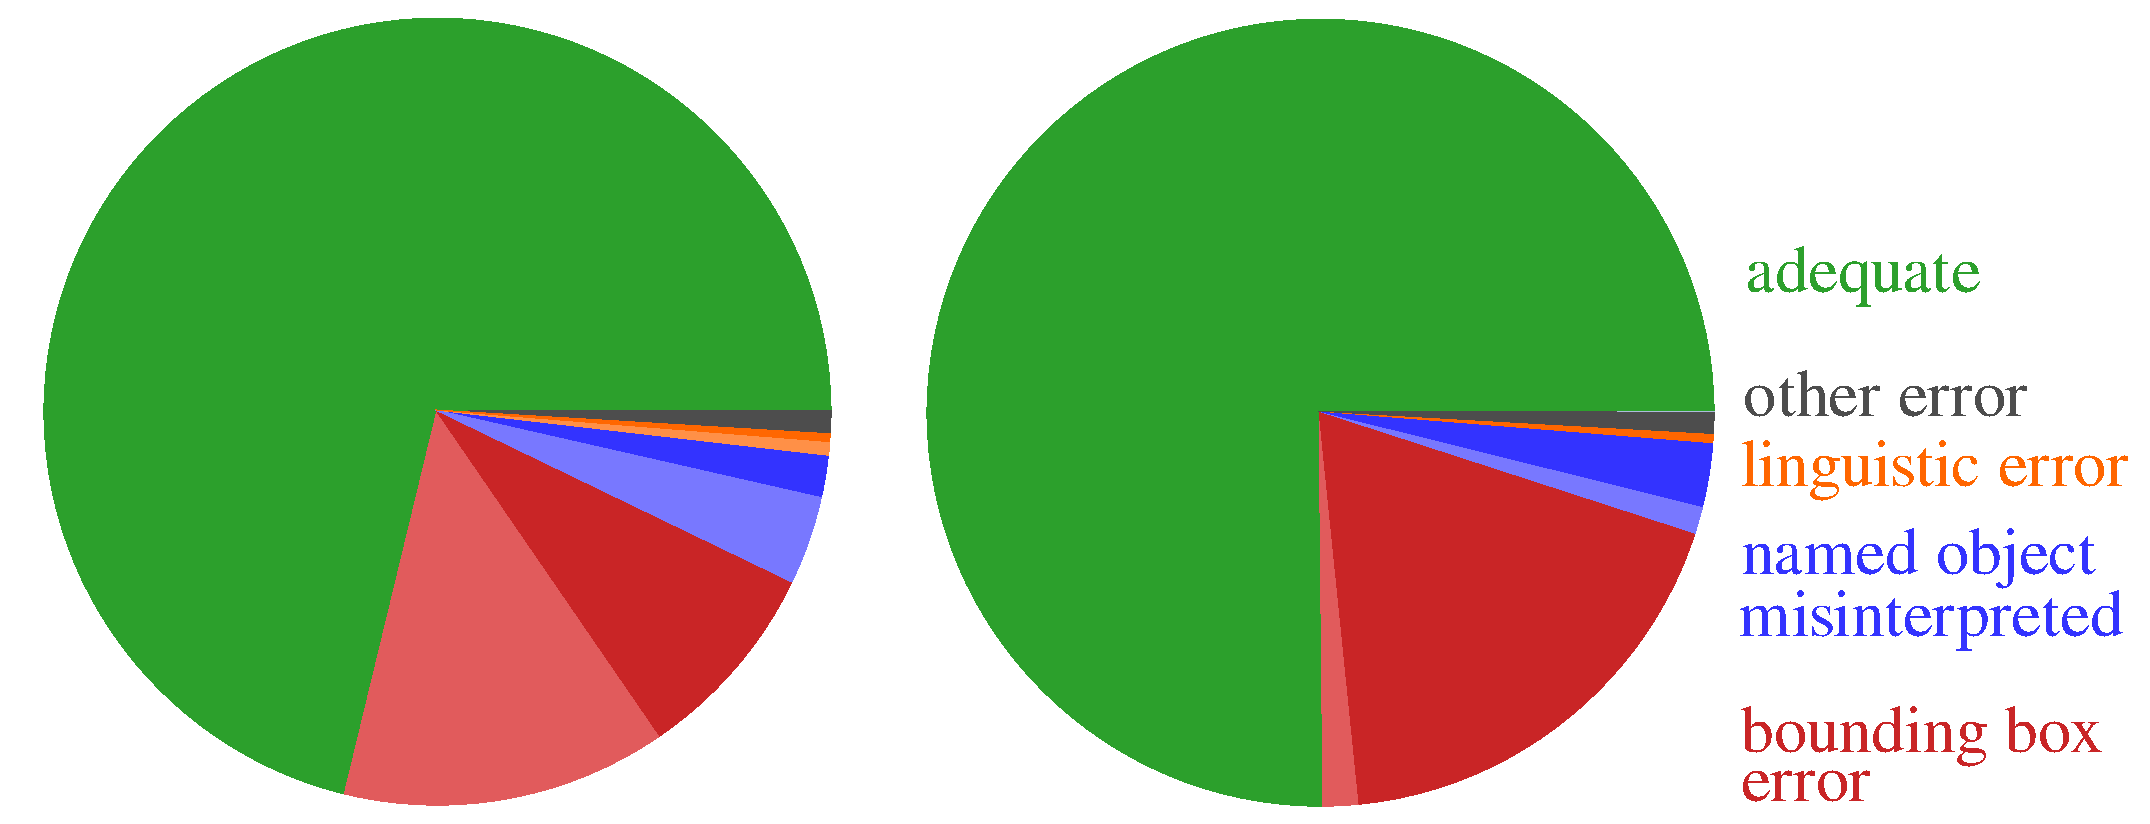
\includegraphics[width=\columnwidth]{images/verification_piechart_double.pdf}\\
% 	\hspace*{\fill}a.\hspace*{\fill}\hspace*{\fill}b.\hspace*{\fill}\hspace*{\fill}
% 	\caption{Verification results: a. counting individual annotations; b. counting image-name pairs with their aggregated scores. Lighter shade within a hue indicates slight/possible error of that type; darker shade severe error.}
% 	\label{fig:verification-piechart}
% \end{figure}


%%% Local Variables:
%%% mode: plain-tex
%%% TeX-master: "acl2020_main"
%%% End:


\section{Experiments}
\label{sec:experiments}
% experiments.tex

\iffalse
\cs{under construction}
\begin{itemize}
	\item Object detection models in CV have different goal than L+V object recognition models (see related work--former is on labels, latter on predicting natural language). 
	However, the former, pre-trained towards labels, are the backbone / used as feature extractors for the latter.
	\item ... 
	\item As we explained, there is a high variation of object names, and objects may be named by multiple alternative names (\cs{vocab size MN vs. vocab size VG for same object set}). 
	Yet, humans usually have a clearly preferred name for individual object instances (and the set of those is relatively small)--humans agree on a particular name for an instance (entry-level name).
	\item Hence, to model human object naming, datasets with many/dozens of annotations for the same instance are required. 
	\item We argue that such datasets are more reliable in that they provide empirically derived preferred names (entry-level names), and richer--the provide valid name alternatives. 
	\item But since their elicitation is expensive and time-consuming, it is not realistic to create training datasets of dozens of object names for pre-training features with CV models, which need a huge amount of training data. 
\end{itemize}
\fi

We propose to use datasets of object names for evaluating models on the task of object naming (depending on results: also valuable for comparing object detection/image classification models).
Specifically, we analyse object detection [and classification] models on the task of human object naming, using the \mn dataset as test data:\\
Can object detection models, trained on arbitrary names, account for human object naming?
\begin{itemize}
	\item Do they predict the entry-level name?
	\item Are valid name alternatives among the top-N predictions?
	\item Do models make similar mistakes as humans when being faced with the task of naming highlighted objects in images [i.e.,\ the artificial setup of object naming for data annotation]?\\
	-- naming an alternative object (maybe more salient)\\
	-- predicting a semantically related name
	%do we get different evaluation results when testing existing object classification models on preferred responses from name distributions, as compared to naming responses collected from 1-3 workers (e.g., VisualGenome)? 
	\item Can we use \mn as fine-tuning dataset? (Here: only Vanilla model)\\
	-- can we learn entry-level names by fine-tuning object detection models on \mn?\\
	-- Can we directly learn entry-level names by fine-tuning image classification models on \mn, i.e.,\ the pre-trained features to initialize object detection models?
\end{itemize}

\subsection{Experimental Setup}
\label{sect:exp_setup}

\paragraph{Data}

\paragraph{Models}

\paragraph{Measures}


\subsection{[TBC] Predicting Entry-Level Names}
\label{sect:exp_entry}
Question: Can object detection models trained on a set of "arbitrarily" chosen object names account for entry-level object names? 

Note that the source dataset for defining the vocabulary (\textsl{Vocab}, i.e.,\ the overall set of considered names, i.e., the softmax layer's dimensions), and the source dataset which provides the ground truth names for the individual objects (\textsl{GTtrain}) may differ.  
\begin{table*}[t]
	\centering
	\small
	\begin{tabular}{l|c|r@{~}r@{~}r@{~}r@{~}r@{~}r@{~}r|@{~}r@{~}r@{~}r@{~}r@{~}r@{~}r@{~}r@{~}}
		\toprule
		&   & \multicolumn{6}{c}{All Test Images ($\#$)} 
		& \multicolumn{6}{c}{VG$\neq$MN Images ($\#$)}\\	
		Model--Vocab	 
		&  GTtrain &  =VG & =MN & $\in$MN  & KL & J & MRR & AvgMRR 
		&  =VG & =MN & $\in$MN  & KL & J & MRR & AvgMRR\\ 
		\midrule
		FRCNN--MN442 & VG &            65.4 &              71.2 &                85.6 &         1.0 &             69.8 &          0.8 &             0.7 &            20.0 &              48.4 &                78.7 &         1.4 &             60.4 &          0.7 &             0.5 \\
		FRCNN--VG2500 & VG \\
		FRCNN--VG1600 & VG &            67.3 &              74.5 &                89.2 &         0.6 &             74.3 &          0.8 &             0.7 &            19.1 &              52.9 &                86.2 &         0.8 &             69.4 &          0.7 &             0.6 \\
		\midrule \midrule
		& \multicolumn{12}{c}{Classifiers: Fine-tuning pre-trained image features on \mn}\\
		Features--Vocab & GTtrain  \\
		\midrule 
		FRCNN--VG1600--VGMN & MN &            70.8 &              80.6 &                90.1 &         4.7 &             62.0 &          0.8 &             0.6 &            13.8 &              60.4 &                85.8 &         4.6 &             47.3 &          0.7 &             0.5 \\ 
		FRCNN--VG1600--MN442 &  MN \\
		\midrule
		ResNet101--VGMN & MN  &            60.9 &              68.6 &                77.9 &         4.9 &             56.4 &          0.8 &             0.6 &            13.8 &              50.2 &                73.3 &         4.7 &             42.9 &          0.6 &             0.4 \\
		
		ResNet101--MN442 & MN &            61.7 &              69.6 &                78.9 &         4.9 &             57.4 &          0.8 &             0.6 &            13.8 &              50.7 &                73.8 &         4.6 &             45.1 &          0.6 &             0.5 \\
		ResNet101--VGMN\_4ep  &   VG &  62.4 &              62.9 &                75.0 &         5.0 &             53.7 &          0.7 &             0.6 &            28.4 &              31.1 &                64.9 &         4.8 &             39.1 &          0.4 &             0.4 \\
		ResNet101--VGMN\_8ep & VG &            63.9 &              62.6 &                75.6 &         5.0 &             53.9 &          0.7 &             0.6 &            34.2 &              28.0 &                66.2 &         4.9 &             39.7 &          0.4 &             0.4 \\
		ResNet101--MN442 & VG  &            63.7 &              63.7 &                76.6 &         5.0 &             55.4 &          0.7 &             0.6 &            30.7 &              31.1 &                67.1 &         4.8 &             41.0 &          0.4 &             0.4 \\
		\bottomrule
	\end{tabular}
	\caption{Target vocabulary in test data: MN442. Vocab denotes the dataset from which the target vocabulary for training was induced (the numbers give the size of the vocabulary). GTtrain denotes the dataset from which the ground truth labels are obtained during \textit{training}. MRR is mean reciprocal rank; J is Jaccard score. Note that we considered all name responses in MN, including those with $\text{count}(name)<2$\label{tab:entrylevels}. }
\end{table*}


\begin{table*}[t]
	\centering
	\small
	\begin{tabular}{l@{~}|rrrr}
		\toprule
		... \\
		\midrule
		Domain	 & ... \\ 
		\midrule
		All           \\
		home           \\
		food           \\
		buildings      \\
		vehicles       \\
		animals\_plants \\
		clothing       \\
		people         \\
		\bottomrule
	\end{tabular}
	\caption{RESULTS FOR SELECTED MODELS \label{tab:domains_bestmodel}}
\end{table*}

\subsection{[TBC] Humans vs. Models: Which Mistakes do they Make?}
\label{sect:exp_analysis}

\paragraph{Categorization of Errors}
see Figure\ ref{fig:mistakes}
\begin{enumerate}
	\item Clear mistake \\
	e.g.,\ rice vs. bread
	\item Alternative name\\
	e.g.,\ building vs. house
	\item Alternative object \cs{(other cluster from verif data)}
	\item Synonym\\
	e.g.,\ plane vs. airplane
	\item Semantically related\\
	e.g.,\  motorcycle vs. scooter
\end{enumerate}

\begin{figure}
	\centering
	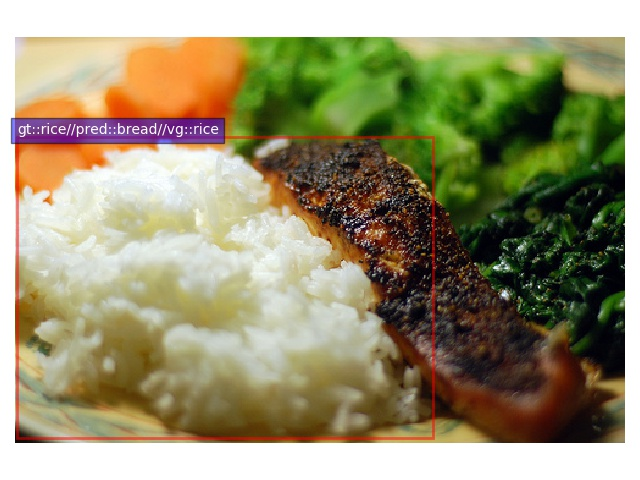
\includegraphics[scale=.2]{images/2323938.jpg}
	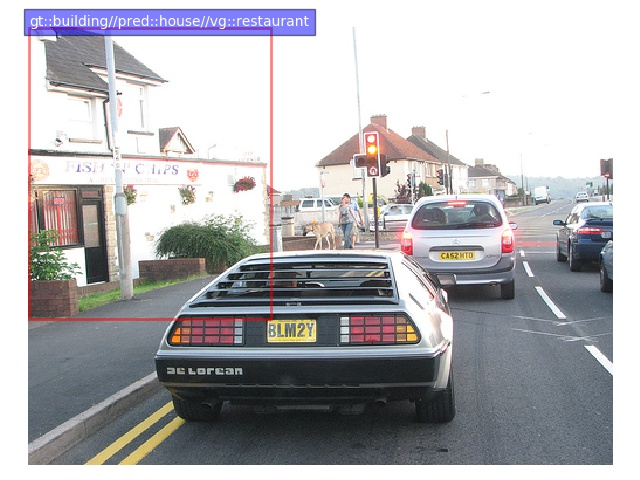
\includegraphics[scale=.2]{images/2322259.jpg}
	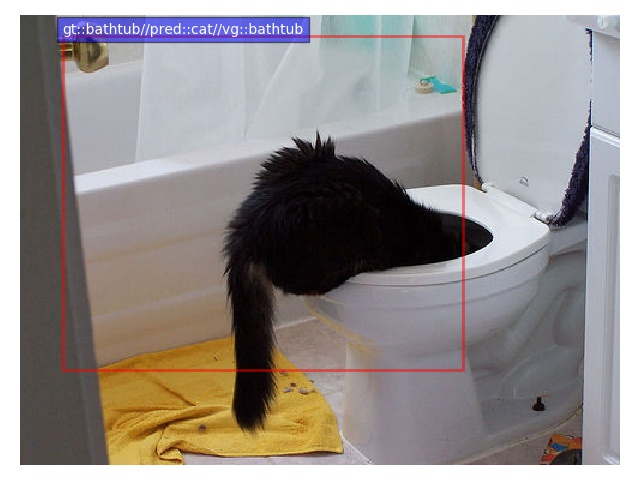
\includegraphics[scale=.2]{images/2371657.jpg}
	
	\caption{resnet mistakes (trained on vg\_manynames, tested on manynames-442)\label{fig:matrices}}
\end{figure}

\subsection{Results}
\paragraph{Overview}
Table\ \ref{tab:exp_overview_results}: \cs{Shows the overview and what MN adds without going into detail: Standard evaluation -- hit; We can additionally distinguish between correct (name alternative, see caption of Table) and clear mistake.}

\paragraph{How do predictions change?} Figure \ref{fig:matrices} visualizes the change in predictions for  some of our retrained and finetuned models with respect to the object detection baseline (bottom-up-1600). For each object, where the new model predicts a different name than the baseline model, we look at the hit-error categories of the original and new predicted name. Observations:
\begin{itemize}
\item Retraining faster-rcnn on less names does not lead to better calibration of entry-level names: more original hits change to same-cluster predictions than the other way round. (top left matrix)
\item Finetuning the original faster-rcnn on many names recalibrates many decision from same-cluster names to the correct hit. Interestingly, also clear errors are calibrated to perfect hits, whereas hardly any error is changed to same-cluster or related.  (top right matrix)
\item A similar tendency can be found for the ResNet models: finetuning ResNet on MN changes many predictions from same-cluster to hits. This is less the case when ResNet is finetuned on VG annotations.
\item Interestingly, both ResNet models change hits into related names (hypernyms, hyponyms, cp-hyponyms) -- why does this happen?
\end{itemize}


\paragraph{Correct predictions}
Table\ \ref{tab:exp_details_correct}: \cs{Gives detailed results to the categories of "correct name" (but not hit): same cluster, WordNet synonym, WordNet hypernym/hyponym}\\
To look into in detail (example images): 
\begin{itemize}
	\item Compare FRCNN vs. FRCNN-finetuned (row block 1 vs. row block 2) with respect to the synonym categories (i.e., predicted name is in a synonym/synonyms\_cluster-relation to the target object) vs. same\_cluster (i.e., predicted name is in response set). 
\end{itemize}

\paragraph{Wrong predictions}

\begin{figure*}[t]
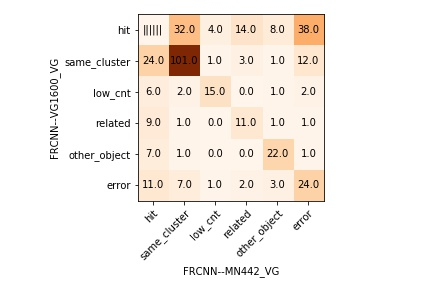
\includegraphics[scale=.5]{images/matrix_FRCNN--VG1600_VG_FRCNN--MN442_VG.jpg}
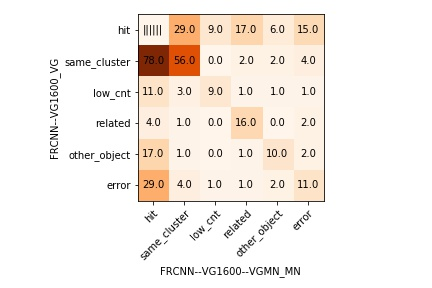
\includegraphics[scale=.5]{images/matrix_FRCNN--VG1600_VG_FRCNN--VG1600--VGMN_MN.jpg}
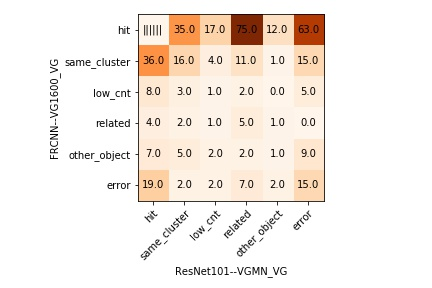
\includegraphics[scale=.5]{images/matrix_FRCNN--VG1600_VG_ResNet101--VGMN_VG.jpg}
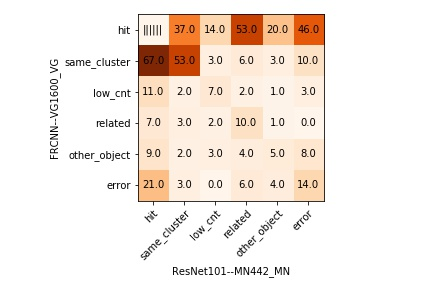
\includegraphics[scale=.5]{images/matrix_FRCNN--VG1600_VG_ResNet101--MN442_MN.jpg}

\caption{Confusion-matrix-style visualization showing error categories of predictions that changed from object detection with FRCNN-VG1600 to naming with FRCNN-VG1600-VGMN (finetuned)}
\end{figure*}



Table\ \ref{tab:exp_details_wrong}: \cs{Gives detailed results to the categories of predicted name\ $\hat{n}$ is incorrect: WordNet co-hyponyms,  other object (inadequacy types: visual, linguistic, bounding box, other (types other+None), $\text{count}(\hat{n})<2$, error (just wrong+unkn(not found in WordNet))}

\begin{table*}[t]
	\centering
	\small
	\begin{tabular}{l|l|r@{~}r@{~}r@{~}||r@{~}r@{~}r@{~}}
		\toprule
		& & \multicolumn{3}{c}{All Test Images ($\#$)} 
		& \multicolumn{3}{c}{VG$\neq$MN Images ($\#$)}\\
	\toprule
	Model--Vocab	& GTtrain  
	&  hit &  correct &  incorrect &  hit &  correct &  wrong \\
	\midrule
	FRCNN--VG1600 & VG           &         74.8 &                  13.9 &                    11.3 &         54.3 &                  30.0 &                    15.7 \\
	FRCNN--MN442 & VG &         71.1 &                  13.9 &                    15.0 &         48.4 &                  28.7 &                    22.9 \\
	\midrule \midrule
	FRCNN--VG1600--VGMN & MN %&         0.81 &                  0.09 &                    0.11 &         0.60 &                  0.23 &                    0.17 \\
	 &         80.7 &                   9.2 &                    10.1 &         60.1 &                  23.8 &                    16.1 \\
	\midrule
	ResNet101--MN442 & MN %& 0.70 &                  0.09 &                    0.21 &         0.51 &                  0.22 &                    0.27 \\
	 &         69.7 &                  10.3 &                    20.1 &         51.1 &                  23.3 &                    25.6 \\
	ResNet101--VGMN & MN% &         0.69 &                  0.09 &                    0.22 &         0.51 &                  0.23 &                    0.26 \\	
	 &         68.7 &                  10.5 &                    20.8 &         50.7 &                  24.2 &                    25.1 \\
	ResNet101--VGMN & VG %&         0.63 &                  0.11 &                    0.26 &         0.31 &                  0.28 &                    0.40 \\
	 &         62.8 &                  12.6 &                    24.6 &         31.4 &                  30.0 &                    38.6 \\
	ResNet101--MN442 & VG %&         0.64 &                  0.11 &                    0.25 &         0.32 &                  0.29 &                    0.39 \\
	 &         63.8 &                  12.6 &                    23.6 &         32.3 &                  30.0 &                    37.7 \\
	\bottomrule
\end{tabular}
\caption{Break-down of the results (in \%): Categorization of a predicted name\ $\hat{n}$ into either a \textit{hit} (exact match with entry-level name, cf. standard evaluation), \textit{correct} (less preferred name, synonym, hypernym/hyponym), or \textit{wrong} (wrong object, $\text{count}(\hat{n})<2$, co-hyponym, clear mistake). \label{tab:exp_overview_results}}
\end{table*}

\begin{table*}[t]
\centering
	\small
\begin{tabular}{lrrr||rrr}
\toprule
&  \multicolumn{3}{c||}{MN agreement $>$ 0.9} & \multicolumn{3}{c}{MN agreement $\leq$ 0.9}\\
                  model &  hit &  correct &  incorrect &  hit &  correct &  incorrect \\
\midrule
       FRCNN--VG1600\_VG &      94.8 &           1.8 &             3.4 &     63.6 &         24.5 &           12.0 \\
        FRCNN--MN442\_VG &      89.6 &           1.6 &             8.8 &     60.7 &         23.9 &           15.4 \\
        		\midrule \midrule
 FRCNN--VG1600--VGMN\_MN &      94.5 &           1.3 &             4.2 &     72.9 &         16.5 &           10.6 \\
 		\midrule 
     ResNet101--VGMN\_VG &      88.3 &           1.8 &             9.9 &     48.5 &         23.6 &           27.8 \\
     ResNet101--VGMN\_MN &      89.6 &           1.6 &             8.8 &     57.0 &         19.4 &           23.6 \\
    ResNet101--MN442\_MN &      90.1 &           1.3 &             8.6 &     58.2 &         19.5 &           22.3 \\
\bottomrule

\end{tabular}
\caption{Break-down of the results (in \%) according to the agreement level of the MN name: Categorization of a predicted name\ $\hat{n}$ into either a \textit{hit}, \textit{correct} (less preferred name, synonym, hypernym/hyponym), or \textit{wrong} \label{tab:errors_agreement}}
\end{table*}


\begin{table*}[t]
	\centering
	\small
	\begin{tabular}{llr@{~}|r@{~}r@{~}r@{~}r@{~}r@{~}||r@{~}|r@{~}r@{~}r@{~}r@{~}r@{~}}
		\toprule
		& & \multicolumn{6}{c}{All Test Images ($\#$)} 
		& \multicolumn{6}{c}{VG$\neq$MN Images ($\#$)}\\
		\toprule
		& &  same &  syn. &  syn. &  hyper. &  hypo. &  hyper. &  same &  syn. &  syn. &  hyper. &  hypo. &  hyper. \\
		& 	&  cluster &  & cluster & & & cluster 
			& cluster  &  & cluster & & & cluster \\
		\midrule
		FRCNN--VG1600 & VG     %        &                  0.95 &              0.0 &                0.01 &              0.01 &             0.03 &                 0.0 &                  0.96 &              0.0 &                 0.0 &              0.01 &             0.03 &                 0.0 \\
		 &                  94.6 &              0.0 &                 0.7 &               3.4 &              1.3 &                  0.0 &                  95.5 &              0.0 &                 0.0 &               3.0 &              1.5 &                  0.0 \\
		FRCNN--MN442 & VG %&                   0.97 &             0.01 &                0.02 &               0.0 &              0.0 &                 0.0 &                  0.97 &              0.0 &                0.03 &               0.0 &              0.0 &                 0.0 \\
		 &                  93.3 &              1.3 &                 2.0 &               1.3 &              2.0 &                  0.0 &                  93.8 &              0.0 &                 3.1 &               1.6 &              1.6 &                  0.0 \\
		\midrule \midrule
		FRCNN--VG1600--VGMN & MN %&                   1.0 &              0.0 &                 0.0 &               0.0 &              0.0 &                 0.0 &                   1.0 &              0.0 &                 0.0 &               0.0 &              0.0 &                 0.0 \\
		 &                  94.9 &              0.0 &                 0.0 &               2.0 &              3.0 &                  0.0 &                  96.2 &              0.0 &                 0.0 &               1.9 &              1.9 &                  0.0 \\
		\midrule
		ResNet101--VGMN & MN %&                  0.97 &              0.0 &                0.03 &               0.0 &              0.0 &                 0.0 &                  0.98 &              0.0 &                0.02 &               0.0 &              0.0 &                 0.0 \\
		 &                  83.9 &              0.0 &                 2.7 &               6.2 &              5.4 &                  1.8 &                  92.6 &              0.0 &                 1.9 &               1.9 &              3.7 &                  0.0 \\
		ResNet101--MN442 & MN %& 0.97 &              0.0 &                0.03 &               0.0 &              0.0 &                 0.0 &                  0.98 &              0.0 &                0.02 &               0.0 &              0.0 &                 0.0 \\
		  &                  86.4 &              0.0 &                 2.7 &               5.5 &              3.6 &                  1.8 &                  92.3 &              0.0 &                 1.9 &               1.9 &              3.8 &                  0.0 \\
		ResNet101--VGMN & VG %&                   0.98 &              0.0 &                0.02 &               0.0 &              0.0 &                 0.0 &                  0.98 &              0.0 &                0.02 &               0.0 &              0.0 &                 0.0 \\
		 &                  87.4 &              0.0 &                 2.2 &               1.5 &              8.1 &                  0.7 &                  92.5 &              0.0 &                 1.5 &               1.5 &              4.5 &                  0.0 \\
		ResNet101--MN442 & VG% &                  0.98 &              0.0 &                0.02 &               0.0 &              0.0 &                 0.0 &                  0.97 &              0.0 &                0.03 &               0.0 &              0.0 &                 0.0 \\		
		&                  88.9 &              0.0 &                 2.2 &               2.2 &              5.9 &                  0.7 &                  92.5 &              0.0 &                 3.0 &               1.5 &              3.0 &                  0.0 \\
		\bottomrule
	\end{tabular}
	
	\caption{Break-down of the results for the \textit{correct} name predictions. Proportions (in \%) of the \textit{correct} categories to all correctly classified instances.  \textit{hyponym}: $\hat{n}$ is a hyponym of the entry-level name. \textit{hypernym\_cl}: $\hat{n}$ is a hypernym of any of the valid names (cluster). \textit{Synonym} and \textit{synonym\_cl} are analogous. \label{tab:exp_details_correct}}
\end{table*}

\begin{table*}[t]
	\centering
	\small
	\begin{tabular}{ll|r@{~}|r@{~}r@{~}r@{~}r@{~}|r@{~}r@{~}||r@{~}|r@{~}r@{~}r@{~}r@{~}|r@{~}r@{~}}
		\toprule
		&& \multicolumn{7}{c}{All Test Images ($\#$)} 
		& \multicolumn{7}{c}{VG$\neq$MN Images ($\#$)}\\
		\toprule
		Model--Vocab & GTtrain  
		&  co- &  \multicolumn{4}{c}{other object}  &  error &  low 
		&  co- &  \multicolumn{4}{c}{other object}  &  error &  low \\
		& & hypo. & (vis. &  ling. &  box &  other)   & & count 
		&  hypo. & (vis. &  ling. &  box &  other) &   & count     \\
		 
	\midrule
	FRCNN--VG1600 & VG     &                 13.2 &             1.7 &                 0.0 &                  17.4 &            6.6 &           39.7 &             21.5 &                  5.7 &             5.7 &                 0.0 &                  17.1 &           14.3 &           42.9 &             14.3 \\
	FRCNN--MN442 & VG       &                 15.5 &             0.6 &                 0.0 &                  15.5 &            6.2 &           49.1 &             13.0 &                  5.9 &             2.0 &                 0.0 &                  13.7 &           11.8 &           54.9 &             11.8 \\
	\midrule \midrule
	FRCNN--VG1600--VGMN & MN &                 30.6 &             0.9 &                 0.0 &                  13.0 &            5.6 &           32.4 &             17.6 &                 16.7 &             2.8 &                 0.0 &                  16.7 &           11.1 &           41.7 &             11.1 \\
	\midrule
	ResNet101--VGMN & MN	&                 34.1 &             0.0 &                 0.0 &                  13.0 &            1.3 &           39.5 &             12.1 &                 19.6 &             0.0 &                 0.0 &                  12.5 &            5.4 &           51.8 &             10.7 \\
	ResNet101--MN442 & MN  &                 33.0 &             0.0 &                 0.0 &                  14.0 &            1.9 &           37.7 &             13.5 &                 21.1 &             0.0 &                 0.0 &                  15.8 &            7.0 &           43.9 &             12.3 \\
	ResNet101--VGMN & VG  &                 37.6 &             0.0 &                 0.0 &                   6.1 &            2.3 &           41.1 &             12.9 &                 24.4 &             0.0 &                 0.0 &                   3.5 &            5.8 &           45.3 &             20.9 \\
	ResNet101--MN442 & VG &                 34.0 &             0.0 &                 0.0 &                   7.5 &            2.8 &           41.9 &             13.8 &                 22.6 &             0.0 &                 0.0 &                   6.0 &            8.3 &           39.3 &             23.8 \\
	\bottomrule
\end{tabular}
\caption{Break-down of the results for the \textit{wrong} name predictions. Proportions (in \%) of the corresponding categories to all wrongly classified instances.  \label{tab:exp_details_wrong}}
\end{table*}




\subsection{[TBC] Generalization Ability: OpenImages}
\label{sect:exp_openimages}
Question: Can models trained towards \mn generalize to other, related datasets? Here: OpenImages. \cs{[Increase coverage with zero-shot learning?]}\

Models compared: FRCNN--VG1600 vs. FRCNN--MN442 vs. ResNet101--XX (best Vanilla).


\section{Conclusions}
\label{sec:conclusions}

%\bibliography{BLA}
%\bibliographystyle{acl_natbib}

%\appendix
%
%\section{Appendices}
%\label{sec:appendix}
%Appendices are material that can be read, and include lemmas, formulas, proofs, and tables that are not critical to the reading and understanding of the paper. 
%Appendices should be \textbf{uploaded as supplementary material} when submitting the paper for review.
%Upon acceptance, the appendices come after the references, as shown here.
%
%\paragraph{\LaTeX-specific details:}
%Use {\small\verb|\appendix|} before any appendix section to switch the section numbering over to letters.
%
%
%\section{Supplemental Material}
%\label{sec:supplemental}
%Supplementary material may report preprocessing decisions, model parameters, and other details necessary for the replication of the experiments reported in the paper.
%Seemingly small preprocessing decisions can sometimes make a large difference in performance, so it is crucial to record such decisions to precisely characterize state-of-the-art methods. 

\bibliographystyle{acl_natbib}
\bibliography{naming}
\end{document}

%%% Local Variables:
%%% mode: latex
%%% TeX-master: "acl2020_main"
%%% End:
